\begin{figure}
  \centering
  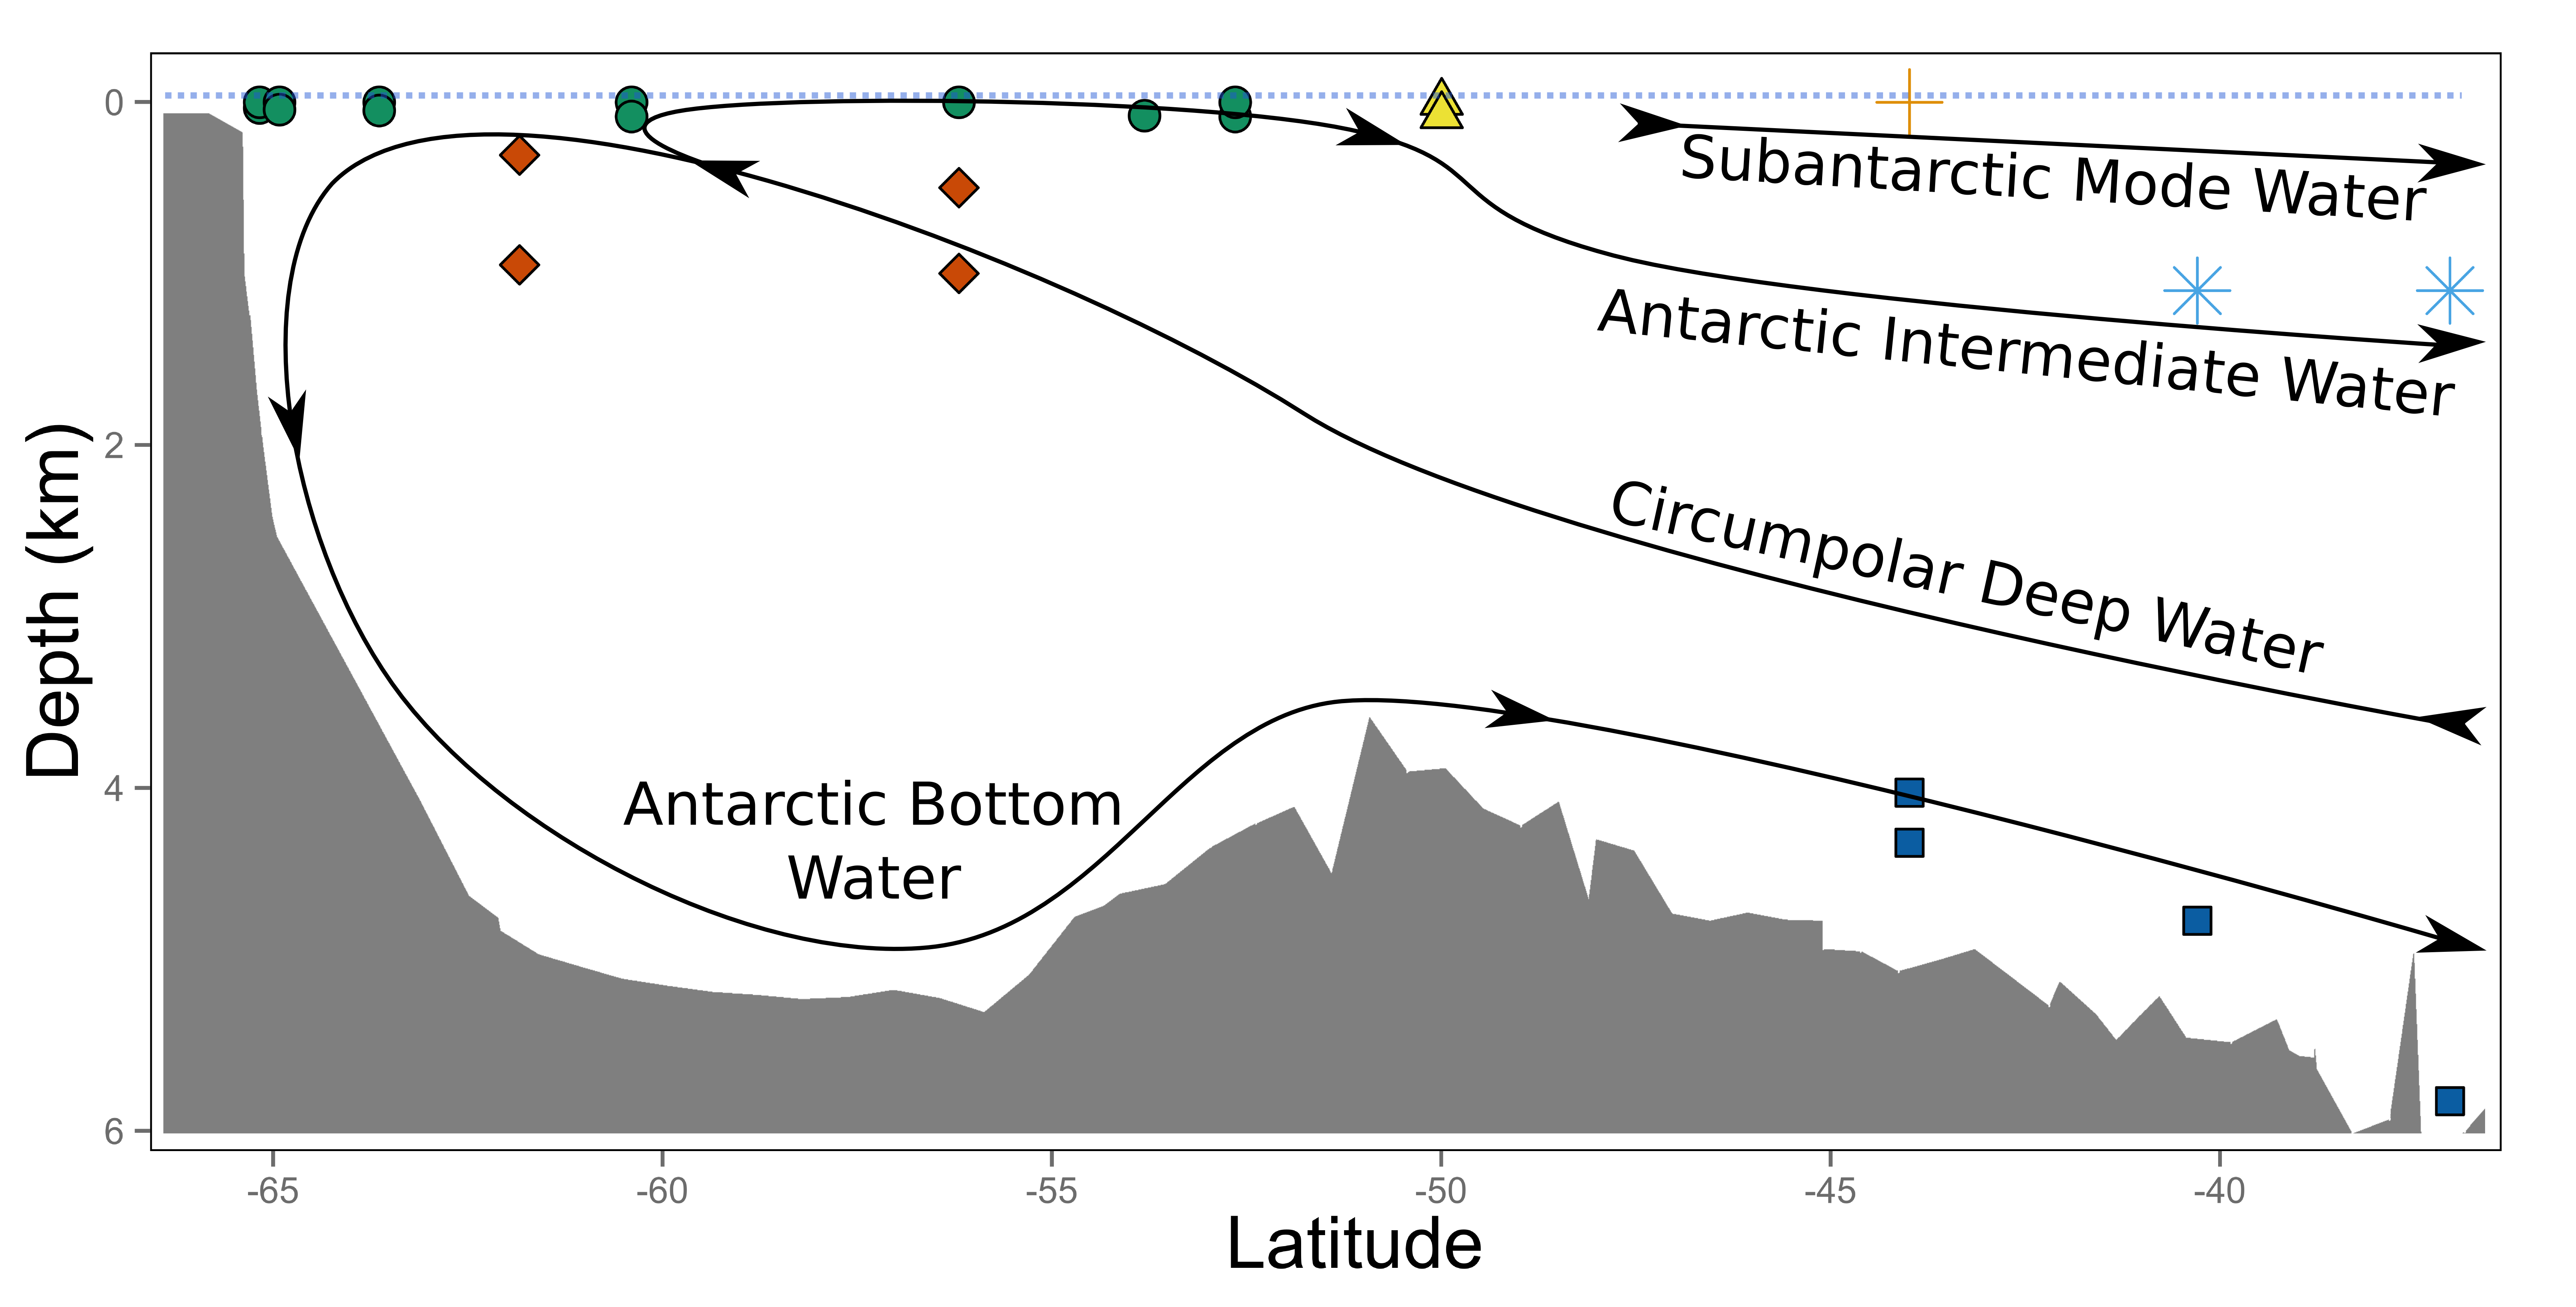
\includegraphics[width=\textwidth]{../advection/advectionsamplemap.png}
  \caption[Map showing sites of samples used in the advection study]{Antarctic Intermediate Waters (AAIW), light blue stars; Subantarctic Mode Water (SAMW), orange crosses; Antarctic Bottom Water (AABW), dark blue squares; Antarctic Zone (AZ), green circles; Polar Frontal Zone (PFZ), yellow triangles; Circumpolar Deep Water (CDW), red diamonds; sea surface, blue dashed horizontal line. Bathymetry is an approximate representation for 115\textdegree{} E, and is indicative only.}
  \label{fig:advectionsamplemap}
\end{figure}
